\begin{figure}[t]
\centering
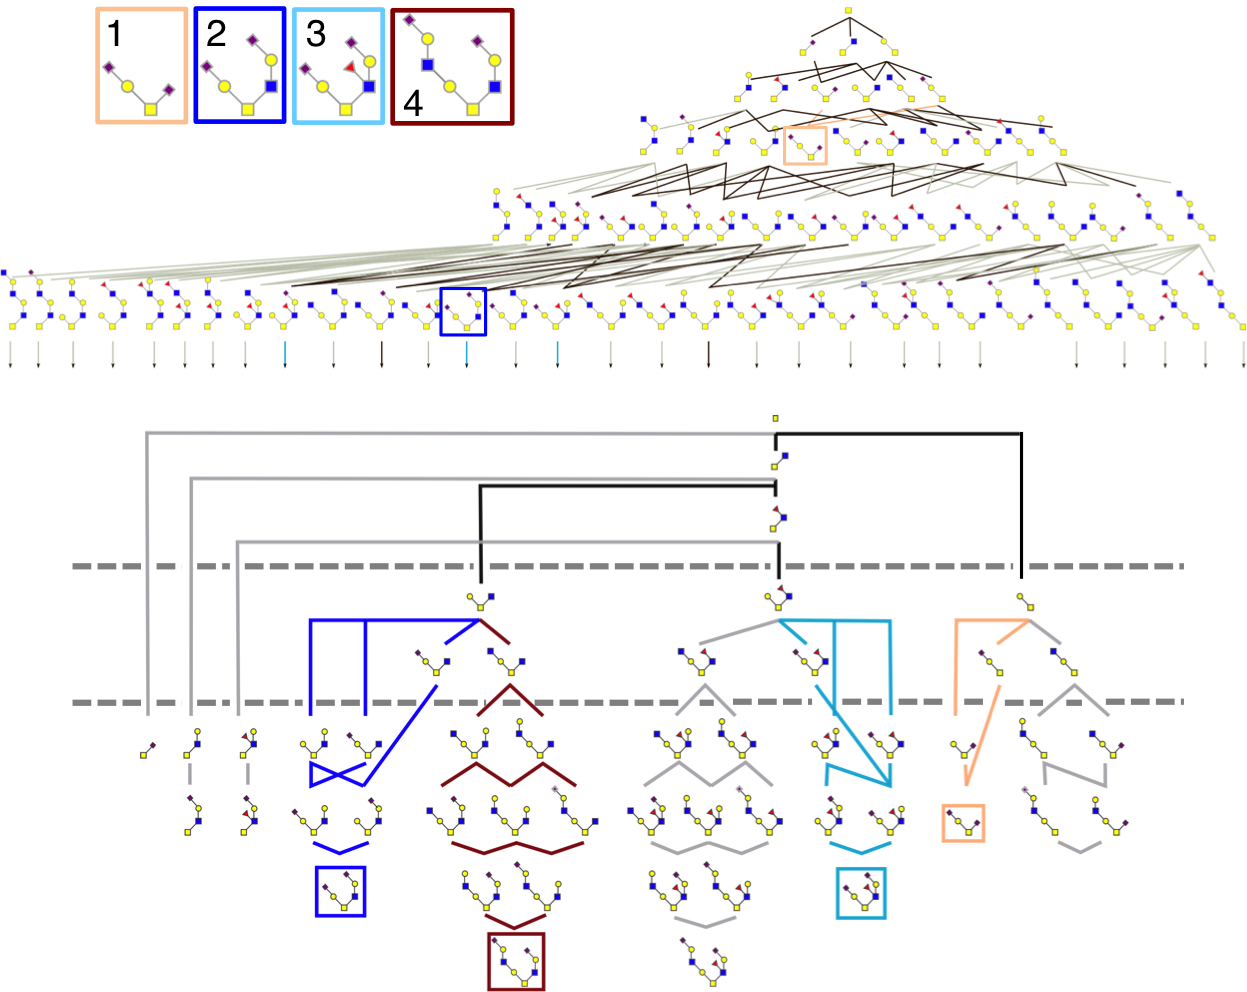
\includegraphics[width=0.8\linewidth]{gfig2.png}
\caption{A glycan data set. Figure credit: Anjali Jaiman, PhD thesis.}
\label{fig:dataset-gly}
\vspace{-6mm}
\end{figure}

\begin{figure}[ht!]
% (sugar a 2)     #Box Yellow
% (sugar c 1)     #Circle yellow
% (sugar b 1)     #Box Blue
% (sugar d 0)     #Diamond red
  \small
  \begin{minipage}{0.5\linewidth}
    \mbox{}
    % \centering
  \begin{tikzpicture}[align at top, shorten >=1pt,thick,node distance=9mm,on grid]
    % (mol (a (c d) d) )
    \node[loc] (v0) {$A$};
    \node[loc, below left of=v0] (v1) {$C$};
    \node[loc, below of=v1] (v2) {$D$};
    \node[loc, below right of=v0] (v3) {$D$};

    \path[->] (v0) edge (v1);
    \path[->] (v1) edge (v2);
    \path[->] (v0) edge (v3);
  \end{tikzpicture}
  \qquad
  \begin{tikzpicture}[align at top, shorten >=1pt,thick,node distance=9mm,on grid]
    % (mol (a (c (b (c d)) ) (b (c d)) ) )
    \node[loc] (v0) {$A$};
    \node[loc, below left of=v0] (v1) {$C$};
    \node[loc, below of=v1] (v2) {$B$};
    \node[loc, below of=v2] (v6) {$C$};
    \node[loc, below of=v6] (v7) {$D$};
    \node[loc, below right of=v0] (v3) {$B$};
    \node[loc, below of=v3] (v4) {$C$};
    \node[loc, below of=v4] (v5) {$D$};

    \path[->] (v0) edge (v1);
    \path[->] (v1) edge (v2);
    \path[->] (v3) edge (v4);
    \path[->] (v4) edge (v5);
    \path[->] (v0) edge (v3);
    \path[->] (v2) edge (v6);
    \path[->] (v6) edge (v7);
  \end{tikzpicture}
  \vspace{-15mm}\par
  \begin{tikzpicture}[align at top, shorten >=1pt,thick,node distance=9mm,on grid]
    % (mol (a (c d) (b (c d)) ) )
    \node[loc] (v0) {$A$};
    \node[loc, below left of=v0] (v1) {$C$};
    \node[loc, below of=v1] (v2) {$D$};
    \node[loc, below right of=v0] (v3) {$B$};
    \node[loc, below of=v3] (v4) {$C$};
    \node[loc, below of=v4] (v5) {$D$};

    \path[->] (v0) edge (v1);
    \path[->] (v1) edge (v2);
    \path[->] (v0) edge (v3);
    \path[->] (v3) edge (v4);
    \path[->] (v4) edge (v5);
  \end{tikzpicture}
  \vspace{-3mm}
  \\
  \mbox{}\hfill(a)\hfill\mbox{}
\end{minipage}
\vrule
  \begin{minipage}{0.48\linewidth}
    \centering
    \begin{tikzpicture}[align at top, shorten >=1pt,thick,node distance=9mm,on grid]
      % 0:(a [(c d)] _)
      \node[loc] (v0) {$A$};
      \node[sqloc, below left of=v0] (v1) {$C$};
      \node[sqloc, below of=v1] (v2) {$D$};
      \path[->] (v0) edge (v1);
      \path[->] (v1) edge (v2);
    \end{tikzpicture}\qquad
    \begin{tikzpicture}[align at top, shorten >=1pt,thick,node distance=9mm,on grid]
      % 0:(a _ [(b-b c)])
      \node[loc] (v0) {$A$};
      \node[sqloc, below right of=v0] (v1) {$B$};
      \node[sqloc, below of=v1] (v2) {$C$};
      \path[->] (v0) edge (v1);
      \path[->] (v1) edge (v2);
    \end{tikzpicture}\qquad\hspace{2ex}
    \begin{tikzpicture}[align at top, shorten >=1pt,thick,node distance=9mm,on grid]
      % 0:(b-b (c [d]))
      \node[loc] (v0) {$B$};
      \node[loc, below of=v0] (v2) {$C$};
      \node[sqloc, below of=v2] (v3) {$D$};
      \path[->] (v0) edge (v2);
      \path[->] (v2) edge (v3);
    \end{tikzpicture}\\\vspace{2ex}
    \begin{tikzpicture}[align at top, shorten >=1pt,thick,node distance=9mm,on grid]
      % 0:(a _ [(d)])
      \node[loc] (v0) {$A$};
      \node[sqloc, below right of=v0] (v1) {$D$};
      \path[->] (v0) edge (v1);
    \end{tikzpicture}
    \quad
    \begin{tikzpicture}[align at top, shorten >=1pt,thick,node distance=9mm,on grid]
      % 0:(a [(c b-b)] (b-b _))
      \node[loc] (v0) {$A$};
      \node[loc, below right of=v0] (v1) {$B$};
      \node[sqloc, below left of=v0] (v2) {$C$};
      \node[sqloc, below of=v2] (v3) {$B$};
      \path[->] (v0) edge (v1);
      \path[->] (v0) edge (v2);
      \path[->] (v2) edge (v3);
    \end{tikzpicture}\qquad
    \begin{tikzpicture}[align at top, shorten >=1pt,thick,node distance=9mm,on grid]
      % 0:(c (b-b [c]))
      \node[loc] (v0) {$C$};
      \node[loc, below  of=v0] (v2) {$B$};
      \node[sqloc, below  of=v2] (v3) {$C$};
      \path[->] (v0) edge (v2);
      \path[->] (v2) edge (v3);
    \end{tikzpicture}
    \\
% % 0:(a _ [b-b])
% % 0:(a _ [d])
% % 0:(a [c] b-b)
% % 0:(c [b-b])
% % 1:(a [c] _)
% % 1:(c [d])
% % 1:(b-b [c])
%     Rules in compartment 1\\
%     \begin{tikzpicture}[align at top, shorten >=1pt,thick,node distance=9mm,on grid]
%       % 0:(a _ [b])
%       \node[loc] (v0) {$A$};
%       \node[sqloc, below right of=v0] (v3) {$B$};
%       \path[->] (v0) edge (v3);
%     \end{tikzpicture}\quad
%     \begin{tikzpicture}[align at top, shorten >=1pt,thick,node distance=9mm,on grid]
%       % 0:(a [c] b)
%       \node[loc] (v0) {$A$};
%       \node[sqloc, below left of=v0] (v1) {$C$};
%       \node[loc, below right of=v0] (v3) {$B$};
%       \path[->] (v0) edge (v1);
%       \path[->] (v0) edge (v3);
%     \end{tikzpicture}\quad
%     \begin{tikzpicture}[align at top, shorten >=1pt,thick,node distance=9mm,on grid]
%       % 0:(a _ [d])
%       \node[loc] (v0) {$A$};
%       \node[sqloc, below right of=v0] (v1) {$D$};
%       \path[->] (v0) edge (v1);
%     \end{tikzpicture}\quad
%     \begin{tikzpicture}[align at top, shorten >=1pt,thick,node distance=9mm,on grid]
%       % 0:(c [b])
%       \node[loc] (v0) {$C$};
%       \node[sqloc, below of=v0] (v1) {$B$};
%       \path[->] (v0) edge (v1);
%     \end{tikzpicture}\\\vspace{2ex}
%     Rules in compartment 2\\
%     \begin{tikzpicture}[align at top, shorten >=1pt,thick,node distance=9mm,on grid]
%       % 1:(a [c] _)
%       \node[loc] (v0) {$A$};
%       \node[sqloc, below left of=v0] (v1) {$C$};
%       \path[->] (v0) edge (v1);
%     \end{tikzpicture}\qquad
%     \begin{tikzpicture}[align at top, shorten >=1pt,thick,node distance=9mm,on grid]
%       % 1:(c [d])
%       \node[loc] (v0) {$C$};
%       \node[sqloc, below of=v0] (v1) {$D$};
%       \path[->] (v0) edge (v1);
%     \end{tikzpicture}\qquad
%     \begin{tikzpicture}[align at top,shorten >=1pt,thick,node distance=9mm,on grid]
%       % 1:(b [c])
%       \node[loc] (v0) {$B$};
%       \node[sqloc, below of=v0] (v1) {$C$};
%       \path[->] (v0) edge (v1);
%     \end{tikzpicture}\\\vspace{2ex}
    (b)
  \end{minipage}
  \hrule
  \begin{minipage}{1.0\linewidth}
    \centering
  \begin{tikzpicture}[align at top, shorten >=1pt,thick,node distance=9mm,on grid]
    % (mol (a (c d) (b (c d)) ) )
    \node[loc] (v0) {$A$};
    % \node[loc, below right of=v0] (v3) {$B$};
    % \path[->] (v0) edge (v3);

    % \node[right of= v3, xshift=-0.2cm] (z1) {$\Rightarrow$};

    % \node[loc, right of= v0, xshift=2.1cm] (v0) {$A$};
    % \node[loc, below left of=v0] (v1) {$C$};
    % \node[loc, below right of=v0] (v3) {$B$};
    % \path[->] (v0) edge (v1);
    % \path[->] (v0) edge (v3);

    \node[right of= v0, yshift=-0.7cm, xshift=-0.2cm] (z2) {$\Rightarrow$};

    \node[loc, right of= v0, xshift=2.1cm] (v0) {$A$};
    \node[loc, below left of=v0] (v1) {$C$};
    \node[loc, below of=v1] (v2) {$D$};
    % \node[loc, below right of=v0] (v3) {$B$};
    \path[->] (v0) edge (v1);
    \path[->] (v1) edge (v2);
    % \path[->] (v0) edge (v3);

    \node[right of= v0, yshift=-0.7cm, xshift=-0.2cm] (z3) {$\Rightarrow$};

    \node[loc, right of= v0, xshift=2.1cm] (v0) {$A$};
    \node[loc, below left of=v0] (v1) {$C$};
    \node[loc, below of=v1] (v2) {$D$};
    \node[loc, below right of=v0] (v3) {$B$};
    \node[loc, below of=v3] (v4) {$C$};
    \path[->] (v0) edge (v1);
    \path[->] (v1) edge (v2);
    \path[->] (v0) edge (v3);
    \path[->] (v3) edge (v4);

    \node[right of= v3, xshift=-0.2cm] (z4) {$\Rightarrow$};

    \node[loc, right of= v0, xshift=2.1cm] (v0) {$A$};
    \node[loc, below left of=v0] (v1) {$C$};
    \node[loc, below of=v1] (v2) {$D$};
    \node[loc, below right of=v0] (v3) {$B$};
    \node[loc, below of=v3] (v4) {$C$};
    \node[loc, below of=v4] (v5) {$D$};
    \path[->] (v0) edge (v1);
    \path[->] (v1) edge (v2);
    \path[->] (v0) edge (v3);
    \path[->] (v3) edge (v4);
    \path[->] (v4) edge (v5);

    % % \node[ below of = z2, yshift=-1cm] (b1) {};
    % \draw [decorate,decoration={brace,amplitude=7pt}]
    % (-0.5,0.5) -- ++(4.5cm,0) node [midway,above,yshift=3pt] {Compartment 1};
    % \draw [decorate,decoration={brace,amplitude=7pt}]
    % (5,0.5) -- ++(8.5cm,0) node [midway,above,yshift=3pt] {Compartment 2};
  \end{tikzpicture}\\
  \vspace{-3mm}
  (c)
\end{minipage}
\hrule
\begin{minipage}{0.2\linewidth}
  \centering
  \begin{tikzpicture}[align at top, shorten >=1pt,thick,node distance=1cm,on grid]
    \node[loc] (v0) {$A$};
    \node[loc, below left of=v0] (v1) {$C$};
    \node[loc, below of=v1] (v2) {$B$};
    \node[loc, below right of=v0] (v3) {$D$};
    \path[->] (v0) edge (v1);
    \path[->] (v1) edge (v2);
    \path[->] (v0) edge (v3);
  \end{tikzpicture}\\
  % \vspace{12ex}
  (d)
\end{minipage}
\vrule
\begin{minipage}{0.75\linewidth}
  \centering
  \begin{tikzpicture}[align at top, shorten >=1pt,thick,node distance=1cm,on grid]
    % 0:(a [(c _)] _)    
    \node[loc] (v0) {$A$};
    \node[sqloc, below left of=v0] (v1) {$C$};
    \path[->] (v0) edge (v1);
  \end{tikzpicture}\qquad
  \begin{tikzpicture}[align at top, shorten >=1pt,thick,node distance=1cm,on grid]
    % 0:(a _ [(b-b c)])
    \node[loc] (v0) {$A$};
    \node[sqloc, below right of=v0] (v1) {$B$};
    \node[sqloc, below of=v1] (v2) {$C$};
    \path[->] (v0) edge (v1);
    \path[->] (v1) edge (v2);
  \end{tikzpicture}\qquad
  \begin{tikzpicture}[align at top, shorten >=1pt,thick,node distance=1cm,on grid]
    % 0:(a _ [(d)])
    \node[loc] (v0) {$A$};
    \node[sqloc, below right of=v0] (v1) {$D$};
    \path[->] (v0) edge (v1);
  \end{tikzpicture}
  % \vspace{-6mm}
  % \\
  \quad
  \begin{tikzpicture}[align at top, shorten >=1pt,thick,node distance=1cm,on grid]
    % 0:(c [(b-b c)])
    \node[loc] (v0) {$C$};
    \node[sqloc, below of=v0] (v1) {$B$};
    \node[sqloc, below of=v1] (v2) {$C$};
    \path[->] (v0) edge (v1);
    \path[->] (v1) edge (v2);
  \end{tikzpicture}\quad
  \begin{tikzpicture}[align at top, shorten >=1pt,thick,node distance=1cm,on grid]
    % 0:(c [(d)])
    \node[loc] (v0) {$C$};
    \node[sqloc, below of=v0] (v1) {$D$};
    \path[->] (v0) edge (v1);
  \end{tikzpicture}\quad
  \begin{tikzpicture}[align at top, shorten >=1pt,thick,node distance=1cm,on grid]
    % 0:[(a (b-b _) _)]
    \node[loc] (v0) {$A$};
    \node[sqloc, below left of=v0] (v1) {$B$};
    \path[->] (v0) edge (v1);
  \end{tikzpicture}
  % % 0:(a _ [b])
  % % 0:(a _ [d])
  % % 1:(a [c] _)
  % % 1:(c [b])
  % % 1:(c [d])
  % % 1:(b [c])
  %   \centering
  %   Rules in compartment 1\\
  %   \begin{tikzpicture}[align at top, shorten >=1pt,thick,node distance=1cm,on grid]
  %     % 0:(a _ [b])
  %     \node[loc] (v0) {$A$};
  %     \node[sqloc, below right of=v0] (v3) {$B$};
  %     \path[->] (v0) edge (v3);
  %   \end{tikzpicture}\quad
  %   \begin{tikzpicture}[align at top, shorten >=1pt,thick,node distance=1cm,on grid]
  %     % 0:(a _ [d])
  %     \node[loc] (v0) {$A$};
  %     \node[sqloc, below right of=v0] (v1) {$D$};
  %     \path[->] (v0) edge (v1);
  %   \end{tikzpicture}\\\vspace{2ex}
  %   Rules in compartment 2\\
  %   \begin{tikzpicture}[align at top, shorten >=1pt,thick,node distance=1cm,on grid]
  %     % 0:(c [b])
  %     \node[loc] (v0) {$C$};
  %     \node[sqloc, below of=v0] (v1) {$B$};
  %     \path[->] (v0) edge (v1);
  %   \end{tikzpicture}\qquad
  %   \begin{tikzpicture}[align at top, shorten >=1pt,thick,node distance=1cm,on grid]
  %     % 1:(a [c] _)
  %     \node[loc] (v0) {$A$};
  %     \node[sqloc, below left of=v0] (v1) {$C$};
  %     \path[->] (v0) edge (v1);
  %   \end{tikzpicture}\qquad
  %   \begin{tikzpicture}[align at top, shorten >=1pt,thick,node distance=1cm,on grid]
  %     % 1:(c [d])
  %     \node[loc] (v0) {$C$};
  %     \node[sqloc, below of=v0] (v1) {$D$};
  %     \path[->] (v0) edge (v1);
  %   \end{tikzpicture}\qquad
  %   \begin{tikzpicture}[align at top,shorten >=1pt,thick,node distance=1cm,on grid]
  %     % 1:(b [c])
  %     \node[loc] (v0) {$B$};
  %     \node[sqloc, below of=v0] (v1) {$C$};
  %     \path[->] (v0) edge (v1);
  %   \end{tikzpicture}\\\vspace{2ex}
    (e)
  \end{minipage}

% \vrule
% \begin{minipage}{0.3\linewidth}
%   \centering
%   \begin{tikzpicture}[align at top, shorten >=1pt,thick,node distance=1cm,on grid]
%     \node[loc] (v0) {$A$};
%     \node[loc, below left of=v0] (v1) {$C$};
%     \node[loc, below of=v1] (v2) {$B$};
%     \node[loc, below of=v2] (v6) {$C$};
%     \node[loc, below of=v6] (v7) {$B$};
%     % \node[loc, below right of=v0] (v3) {$B$};

%     \path[->] (v0) edge (v1);
%     \path[->] (v1) edge (v2);
%     % \path[->] (v3) edge (v4);
%     % \path[->] (v4) edge (v5);
%     % \path[->] (v0) edge (v3);
%     \path[->] (v2) edge (v6);
%     \path[->] (v6) edge (v7);
%     \draw [decorate,decoration={brace,amplitude=7pt}]
%     (-0.3cm,-2cm) -- ++(0cm,-2cm) node [midway,right,xshift=2mm]
%     {Repeated pattern};
%   \end{tikzpicture}\\
%   (e)
% \end{minipage}
  
  \vspace{-3mm}
  \caption{(a) A schematic example of a data set that includes three glycan oligomers.
    % Note that we have used a convention of keeping the root on top, which is opposite to the biological convention of keeping the root at the bottom.
    (b) A set of production rules for the glycan molecules
    (c) The steps of producing the middle glycan molecule
    (d) An undesired molecule.
    % The conditions on siblings help us avoid producing it.
    % (e) Another undesired molecule.
    % The conditions on ancestors help us avoid producing it.
    (e) the synthesized rules at the first iteration.
  }
  \label{fig:ex-gly}
  \vspace{-9mm}
\end{figure}

%%% Local Variables:
%%% mode: latex
%%% TeX-master: "main"
%%% End:


In this section, we first present a motivating example to illustrate our method.
In Figure~\ref{fig:dataset-gly},
we consider the glycan oligomers associated with human chorionic
gonadotropin~\cite{Harrd1992}.
The data set has four glycan oligomers (shown in boxes and numbered). If we assume that all these oligomers
are built by starting from a root GalNAc (yellow square) by adding one monomer at a
time (lines between glycans represent monomer addition reactions). At the top of the figure, we illustrate
if all enzymes (rules) operate in a
single compartment, a large number of glycans can potentially be made in addition to the measured ones.
In the lower part of the figure, we illustrate if the enzymes are split into three compartments
(separated by dotted lines), then certain reactions are prevented from occurring, so the set of structures
made is reduced.
In this case, we assume that only the terminal (bottom-most) structures will be produced as outputs.
Here we have assumed certain rules of operation that are most consistent with the observed glycan data set.
The goal of this paper is to infer the rules.


Now we may consider the abstract general problem. In Figure~\ref{fig:ex-gly}(a), we present a set of
glycan molecules present in a cell consists of three molecules, which are structurally similar to the
three glycan molecules in Figure~\ref{fig:dataset-gly}.
To keep things simple for illustration, we have dropped the third glycan molecule
(inside light blue square) from the four in
Figure~\ref{fig:dataset-gly}.
%
The molecules contain four types of monomers.
As we are considering the abstract case, we have named them $A$, $B$, $C$, $D$.
Each monomer is associated with an arity, i.e., the maximum number of potential children.
The arities of the monomers are $2$, $1$, $1$, and $0$, respectively.

Before considering the synthesis problem that produces exactly
the three molecules,
let us consider a set of rules in Figure~\ref{fig:ex-gly}(b)
that produce the molecules.
There are six rules.
All the rules are in the same compartment.
% The first compartment has four rules and the second compartment has three rules.
The rules have two kinds of nodes.
If the circular nodes are present around a leaf,
the rule is enabled and appends the molecule at the leaf with the square nodes.
In Figure~\ref{fig:ex-gly}(c), we show the steps of generating the middle
glycan molecule.
The first two steps add two nodes at a time.
The last step looks at the two ancestors before adding a single node.
We may avoid the need for compartments if the operations can add multiple nodes at
a time or look for a deep context for being enabled.

The second last rule in Figure~\ref{fig:ex-gly}(b) has a non-trivial condition
on the sibling of the anchor leaf node.
It requires, the parent of the new node should be $A$ and the right sibling
must be $B$.
If we do not have the sibling condition, we may be able to construct the molecule
in Figure~\ref{fig:ex-gly}(d) using the fourth and the modified fifth rule.
The molecule is not in a subtree of any of the three input glycan molecules.
Therefore, there are scenarios where rules must look into the context before applying
themselves.

Furthermore, there is another interesting case occurs in this example.
Please look at the last two rules.
The second last rule adds $C\rightarrow B$ branch.
The last rule checks if $C\rightarrow B$ nodes are present then adds $C$.
If both rules were adding one node at a time without checking deep context,
then the undesired molecule pattern in Figure~\ref{fig:ex-gly}(e) is
also producible.
We would have needed compartments to avoid the undesirable molecule.
Therefore, there is a tread-off between rule sizes and the number of compartments.


Our method for synthesis takes the three glycan molecules as input.
It also needs the budget of resources to search for the production rules.
If we allow an arbitrary number of rules,
the rules to look at their context up to
an arbitrary depth, and an arbitrarily large number of compartments,
then there is a trivial solution.
Therefore, our method needs three parameters.
The first parameter limits the number of rules.
The second parameter limits the maximum height of the rule trees.
The third parameter limits the maximum number of compartments.
If we give larger values to the parameters, then we have more chances to
find the production rules.
For this illustration, we searched for the production rules with
seven as the limit on the number of rules, three as the limit on the rule heights,
and a single compartment.

\ourtool, the tool that implements the method, reported the synthesized rules from
Figure~\ref{fig:ex-gly}(b) in 0.4 seconds.
In our tool, we first construct a synthesis query using the templates to encode
that a set of rules produces the input molecules.
We call a solver to solve the synthesis query.
After the first query, we obtain the rules presented in Figure~\ref{fig:ex-gly}(f).
Next, we look for another molecule that may be produced by the rule.
Using another query to the solver, we find a counterexample molecule that is
producible by the rules but is not in the input set.
Coincidently, we have already presented the counterexample molecule in Figure~\ref{fig:ex-gly}(e).
Afterword, we add constraints that the molecule must not
be producible by the synthesized rules in our synthesis query and go for the next iteration.
After 19 iterations, our tool synthesizes a set of rules that satisfies the requirements.


%--------------------- DO NOT ERASE BELOW THIS LINE --------------------------

%%% Local Variables:
%%% mode: latex
%%% TeX-master: "main"
%%% End:
